\documentclass[]{article}
\usepackage{lmodern}
\usepackage{amssymb,amsmath}
\usepackage{ifxetex,ifluatex}
\usepackage{fixltx2e} % provides \textsubscript
\ifnum 0\ifxetex 1\fi\ifluatex 1\fi=0 % if pdftex
  \usepackage[T1]{fontenc}
  \usepackage[utf8]{inputenc}
\else % if luatex or xelatex
  \ifxetex
    \usepackage{mathspec}
  \else
    \usepackage{fontspec}
  \fi
  \defaultfontfeatures{Ligatures=TeX,Scale=MatchLowercase}
\fi
% use upquote if available, for straight quotes in verbatim environments
\IfFileExists{upquote.sty}{\usepackage{upquote}}{}
% use microtype if available
\IfFileExists{microtype.sty}{%
\usepackage{microtype}
\UseMicrotypeSet[protrusion]{basicmath} % disable protrusion for tt fonts
}{}
\usepackage[margin=1in]{geometry}
\usepackage{hyperref}
\hypersetup{unicode=true,
            pdftitle={Detecting marine heatwaves with sub-optimal data},
            pdfauthor={Robert W. Schlegel(1,2), Eric C. J. Oliver(1), Alistair J. Hobday(3), Albertus J. Smit(2)},
            pdfborder={0 0 0},
            breaklinks=true}
\urlstyle{same}  % don't use monospace font for urls
\usepackage{graphicx,grffile}
\makeatletter
\def\maxwidth{\ifdim\Gin@nat@width>\linewidth\linewidth\else\Gin@nat@width\fi}
\def\maxheight{\ifdim\Gin@nat@height>\textheight\textheight\else\Gin@nat@height\fi}
\makeatother
% Scale images if necessary, so that they will not overflow the page
% margins by default, and it is still possible to overwrite the defaults
% using explicit options in \includegraphics[width, height, ...]{}
\setkeys{Gin}{width=\maxwidth,height=\maxheight,keepaspectratio}
\IfFileExists{parskip.sty}{%
\usepackage{parskip}
}{% else
\setlength{\parindent}{0pt}
\setlength{\parskip}{6pt plus 2pt minus 1pt}
}
\setlength{\emergencystretch}{3em}  % prevent overfull lines
\providecommand{\tightlist}{%
  \setlength{\itemsep}{0pt}\setlength{\parskip}{0pt}}
\setcounter{secnumdepth}{0}
% Redefines (sub)paragraphs to behave more like sections
\ifx\paragraph\undefined\else
\let\oldparagraph\paragraph
\renewcommand{\paragraph}[1]{\oldparagraph{#1}\mbox{}}
\fi
\ifx\subparagraph\undefined\else
\let\oldsubparagraph\subparagraph
\renewcommand{\subparagraph}[1]{\oldsubparagraph{#1}\mbox{}}
\fi

%%% Use protect on footnotes to avoid problems with footnotes in titles
\let\rmarkdownfootnote\footnote%
\def\footnote{\protect\rmarkdownfootnote}

%%% Change title format to be more compact
\usepackage{titling}

% Create subtitle command for use in maketitle
\newcommand{\subtitle}[1]{
  \posttitle{
    \begin{center}\large#1\end{center}
    }
}

\setlength{\droptitle}{-2em}

  \title{Detecting marine heatwaves with sub-optimal data}
    \pretitle{\vspace{\droptitle}\centering\huge}
  \posttitle{\par}
    \author{Robert W. Schlegel(1,2), Eric C. J. Oliver(1), Alistair J. Hobday(3),
Albertus J. Smit(2)}
    \preauthor{\centering\large\emph}
  \postauthor{\par}
      \predate{\centering\large\emph}
  \postdate{\par}
    \date{April 30th, 2018}


\begin{document}
\maketitle

1: Department of Oceanography, Dalhousie University, Halifax, Nova
Scotia, Canada 2: Department of Biodiversity and Conservation Biology,
University of the Western Cape, Bellville, South Africa 3: CSIRO Oceans
and Atmosphere, Hobart, Tasmania, 7000, Australia

\hypertarget{abstract}{%
\section{Abstract}\label{abstract}}

Marine heatwaves (MHWs), or prolonged periods of anomalously warm sea
water temperature, have been increasing in duration and intensity
globally for decades. However, there are many coastal, oceanic, and
polar regions where our ability to detect MHWs is uncertain due to the
unavailability of high-quality data. Here we investigate the effect that
short time series length, missing data, or linear decadal temperature
trends may have on the detection of MHWs. We show that MHWs detected in
time series as short as 10 years did not have durations or intensities
significantly different from the same events detected in a standard
length 30 year time series, but the accurate identification of
temperature thresholds could be impaired when fewer than 15 years of
data were used. We also show that for time series missing less than 20\%
data, the intensity-based MHW categories did not differ significantly
from those detected in complete time series. Linear decadal trends of
0.05 -- 0.15°C/dec could lead to inaccurate creation of seasonal
climatologies, but this did not impact accurate MHW detection. The
percentage of missing data in a time series was determined to have the
largest effect on the detection of MHWs, but was also the easiest to
correct for. Time series length had less of an effect on MHW detection,
but was more difficult to correct for. We provide suggestions for best
practices to improve the accuracy of MHW detection with sub-optimal time
series on a global scale and specific case studies of three notable MHWs
from the literature.\\
(xxx words)

\hypertarget{introduction}{%
\section{Introduction}\label{introduction}}

The idea of locally warm seawater being problematic is not a novel
concept. We have known for decades that seemingly transient warm water
occurrences in the ocean could result in major impacts (e.g. Baumgartner
1992, @Salinger2016). The study of the effects of anomalously warm
seawater temperatures began in earnest in the early 1980's when research
into the ENSO phenomenon began (e.g. Philander 1983). After the 1980's,
researchers began noticing that warm water events were becoming more
frequent and problematic, but it wasn't until 2018 that this was
demonstrated with global observations (Oliver et al. 2018).

In order to quantify the increased occurrence and severity of these
events it was necessary to develop a methodology that would be
inter-comparable for the entire planet. This was accomplished in 2016
after the International Working Group on Marine Heatwaves
(marineheatwaves.org) initiated a series of workshops to address this
issue (Hobday et al. 2016). This definition for anomalously warm
seawater events, known as marine heatwaves (MHWs), has seen wide-spread
and rapid adoption due to ease of use and applicability to any part of
the globe. One problem with this algorithm that has not yet been
addressed is the assumption that a researcher has access to the highest
quality data available when detecting MHWs. In the context of MHW
detection `high quality' is a daily time series with no missing data
that is at least 30 years in length. To avoid contention on the use of
the word `quality', time series that meet the aforementioned standard
are referred to here as `optimal', whereas those that do not meet some
part of the standard are referred to as `sub-optimal'.

Most remotely-sensed data, and more recently output from ocean models
and reanalyses, consist of over 30 years of data and utilise statistical
techniques to fill gaps in the time series from a number of
environmental and technical sources. This means that these data are
considered optimal for MHW detection however, they still have issues
(e.g.~land bleed and incorrect data flagging) and so it may be
recommended that researchers utilise sub-optimal data when possible,
such as sporadically collected \emph{in situ} time series. Coastal areas
are often poorly sampled yet are the most susceptible to the impacts of
MHWs (e.g. Smale et al. 2019) so it is necessary to address the issues
that using these data may have on the detection of MHWs.

This paper seeks to understand the limitation of using sub-optimal data
for the detection of MHWs. Of primary interest are three key challenges:
1) The use of short time series, 2) the use of time series with missing
data, 3) the use of time series in areas with large decadal temperature
trends. We will use a combination of reference time series from specific
locations and global data to address these issues. The effects of the
three sub-optimal data challenges on the detection of MHWs are
quantified in order to provide researchers with the level of confidence
they may express in their results. Where possible, best practices for
the correction of these issues are detailed.

\hypertarget{defining-marine-heatwaves}{%
\section{Defining marine heatwaves}\label{defining-marine-heatwaves}}

The definition used in this paper for a MHW is ``a prolonged discrete
anomalously warm water event that can be described by its duration,
intensity, rate of evolution, and spatial extent.'' (Hobday et al.
2016). This qualitative definition is quantified with an algorithm that
calculates a suite of metrics. These metrics may then be used to
characterise MHWs and to effectively compare them against known
ecological/financial impacts. The calculation of these metrics is made
possible by first determining the mean and 90th percentile temperature
for each of the 366 calendar day-of-year (doy) in a time series. The
mean doy temperatures, which also represent the seasonal signal in the
time series, provide the expected baseline temperature whose daily
exceedance is used to calculate the intensity of MHWs. The 90th
percentile doy temperatures serve as the threshold that must be exceeded
for 5 or more consecutive days for the anomolously warm temperatures to
be classified as a MHW and for the caluclation of the MHW metrics to
begin.

In this paper we will focus on the two metrics that most succinctly
summarise a MHW. The first metric, \emph{duration (days)}, is defined as
the number of days that the temperature remains at or above the 90th
percentile threshold without dipping below it for more than 2
consecutive days. The duration of an event is the best single
measurement of the chronic stress that a MHW may inflict upon a target
sepcies or ecosystem. The second metric, \emph{maximum intensity (°C)},
is the single warmest day during the event and is calculated by
subtracting the mean doy temperature on that day from the recorded
temperature. This metric is the best single representation of acute
stress. There are many other MHW metrics and the full explanation for
them may be found in Table 2 of Hobday et al. (2016).

Hobday et al. (2018) extended the MHW definition to include a
categorisation scheme based on the intensity of an event. These
categories were: I Moderate, II Stong, III Severe, and IV Extreme. The
category of an event is determined by how many times the maximum
intensity of the MHW is a multiple of the difference between the mean
and 90th percentile doy temperatures. For example, if the difference
between the mean and 90th percentile doy temperatures on the warmest day
of a MHW 1.5°C, and the temperature recorded on that warmest day was 3°C
warmer than the mean doy temperature for that day, this would be
considered a category II (Strong) MHW. Were the maximum temperature
recorded at 4.5°C, this would then be classified as a category III
Severe MHW. To provide a more robust qualificatin of a MHW, the
categories are also calculated for each day of a MHW to provide a
proportion of the days during which the event was within each of the
categories.

An additional advantage in the use of the Hobday et al. (2016) and
Hobday et al. (2018) approach is that it has been developed for python
(\url{https://github.com/ecjoliver/marineHeatWaves}), R (Schlegel and
Smit 2018), and MATLAB (Zhao and Marin 2019). For this analysis we
compared the R and python default outputs, assessed how changing the
arguments affected the results, and compared the other functionality
provided between the two languages. While some style differences exist
between the added functionality of the languages, the core climatology
outputs are identical to within \textless{} 0.001 °C per day-of-year
(doy). An independent analysis of the Python and MATLAB results also
confirmed that they were functionally identical (pers. com. Zijie Zhao;
MATLAB distribution author).

\hypertarget{what-are-optimal-data-for-detecting-marine-heatwaves}{%
\section{What are optimal data for detecting marine
heatwaves?}\label{what-are-optimal-data-for-detecting-marine-heatwaves}}

Hobday et al. (2016) stated that optimal data for detecting MHWs have
the following porperties: 1) the time series must be at least 30 years
in length, 2) be quality controlled, 3) be of the highest resolution
possible, and 4) \emph{in situ} data should be used to compliment
remotely sensed data where possible. Whereas the authors did not
specifically state that time series must not contain large proportions
of missing data, it can be inferred from the aforementioned
requirements. There are a number of methods within the already existing
tools for detecting MHWs that can address these concerns and we will lay
them out here. An issue not discussed in Hobday et al. (2016) is the
effect of long-term trends on the accurate detection of events. Oliver
et al. (2018) have shown how dominant the climate change signal can be
in the detection of events and we seek to quantify this effect here.

A time series with a sub-optimal length may impact the detection of MHWs
by negatively affecting the creation of the daily climatology relative
to which MHWs are detected in two primary ways. The first is that with
fewer years of data to draw from, the presence of an anomalously warm or
cold year will have a larger effect on the climatology than with a
sample size of 30 years. The second cause is that because the world is
generally warming (Pachauri et al. 2014), the use of a shorter time
series will almost certainly warm bias the results.

The climatology derived from a time series serves two main roles
(Organization 2017); 1) it serves as a `benchmark' relative to which
past and future measurements can be compared, and against which
anomalies can be calculated, 2) it reflects the typical conditions
likely to be experienced at a particular place at a particular time. The
WMO Guide to Climatological Practices (Organization 2011) stipulate that
daily climatologies (which they call `climate normal') must be based on
the most recent 30-year period that ends on a complete decade (currently
1981 -- 2010). It is from this WMO guideline that the optimal length for
MHW detection was derived.

Some remotely sensed products suffer from `gappiness' that result in
missing data being introduced. This may be due to cloud cover, the
presence of sea ice, unsuitable sea states, etc., which become more
prevalent at smaller scales, particularly nearer the coast. Some
products smooth out these influences, but this results in smoothed SST
fields that mask some of the small-scale spatial variation in surface
temperatures. Other times they rely on blending with data from other
products, which may have its own suite of consequences. This is why the
use of imperfect \emph{in situ} collected time series may still be
encouraged in certain situations. These data are however also prone to
large gaps and so the problems these data face with regards to accurate
event detection are generally uncertain.

\hypertarget{do-i-have-enough-data}{%
\section{Do I have enough data?}\label{do-i-have-enough-data}}

In order to quantify the effects that time series length, missing data,
and decadal trends have on MHW detection we will focus on the following
three items:

\begin{enumerate}
\def\labelenumi{\arabic{enumi})}
\tightlist
\item
  The climatologies derived from the daily SST records, which include
  both the seasonally-varying mean and 90th percentile threshold.

  \begin{itemize}
  \tightlist
  \item
    These are not a part of the MHWs themselves, but are necessary fo
    their detection.
  \end{itemize}
\item
  The MHW event itself, which is defined by the metrics given in Table 2
  of Hobday et al. (2016).

  \begin{itemize}
  \tightlist
  \item
    We chose here to focus on only the duration (days) and maximum
    intensity (°C) metrics in order to keep the results manageable.
  \end{itemize}
\item
  The proportion of days of the event that are within the different
  categories.

  \begin{itemize}
  \tightlist
  \item
    These are a more qualitative result that may be more applicable to a
    broader audience.
  \end{itemize}
\end{enumerate}

With these three focal items defined, we then used the following three
questions to frame the results:

\begin{enumerate}
\def\labelenumi{\arabic{enumi})}
\tightlist
\item
  How sub-optimal can data be before any of the above three items become
  significantly different from those calculated with an optimal time
  series?

  \begin{itemize}
  \tightlist
  \item
    For example, how short may a time series be before the climatology
    becomes significantly different from the same climatology derived
    from the full 30 year time series?
  \end{itemize}
\item
  What amounts of uncertainty are introduced into the results from the
  increasingly sub-optimal data?

  \begin{itemize}
  \tightlist
  \item
    For example, when 20\% of data are missing, what should a user
    expect the standard error around the duration of a MHW to be
    compared to that same MHW when detected in a time series mising no
    data?
  \end{itemize}
\item
  Are the error rates introduced by sub-optimal data the same/similar
  everywhere in the world, or do they differ based on some observable
  pattern/known oceanographic feature(s)?

  \begin{itemize}
  \tightlist
  \item
    For example, when the length of a time series is shortened to 10
    years in an eastern boundary upwelling system (EBUS), does the
    effect this have on the maximum intensity of the events differ form
    the same shortening on a time series in a western boundary current
    (WBC)?
  \end{itemize}
\end{enumerate}

In the following sub-sections we will describe how we control for the
three sub-optimal time series challenges and outline how we ensured that
one could (or could not) use these data in the face of these challenges.
In order to answer these questions we will use the remotely sensed NOAA
OISST dataset (Reynolds et al. 2007, Banzon2016). This remotely-sensed
SST product has a spatial resolution of 1/4 degree globally, and a daily
temporal resolution. The first complete year of data available is 1982,
meaning that we must deviate slightly from the WMO standard for daily
climatology creation by setting our reference period at 1982 -- 2011.

\hypertarget{assessing-the-effect-of-time-series-length}{%
\subsection{Assessing the effect of time series
length}\label{assessing-the-effect-of-time-series-length}}

In order to determine at what number of years MHWs detected in shortened
time series become significantly different from an assumed truth, based
on a standard 30-year record, we first remove the long-term linear
trends in the data before systematically shortening the reference time
series one year at a time, from the maximum length currently available
length of 37 years in the NOAA OISST dataset (first complete year of
data is 1982), down to a minimum length of ten years (start date of
2009, end date of 2018), before comparing the results with a
Kolmogorov-Smirnov test. This test is designed specifically to look for
differences in the distribution of values between two sets of data,
rather than testing for differences of central tendency (e.g.~t-test or
ANOVA). It was decided to not test for central tendency as the
assumption that the results were normally distributed was usually
violated.

In order to make this analysis more robust, the above methodology was
also performed on each reference time series with the order of the years
randomly re-sampled and recombined 100 times. We chose this method
instead of creating artificial time series with comparable
auto-correlation structures as it ensured that the large historical MHWs
present in the reference time series could still be accounted for as
these are an important reason why these time series were chosen. Because
it would violate the assumption of equitable sample sizes were we to
compare events from a 30 year time series against a much shorter time
series, we have limited the length of the shortest time series being
compared to 10 years and compare only events from the different lengths
of time series that only occurred in the most recent 10 years. This was
so that we could still have a reasonable sample size to draw from as we
could only compare the results from time series of varying lengths for
years in which they overlapped. Because the lengths of the time series
were being varied, it was also necessary that the climatology period
vary likewise. To maintain as much consistency as possible across the
results we used the full range of years within each shortened time
series to determine the climatology. For example, if the time series had
been shortened from 37 to 32 years (1987 -- 2018), the 32 year period
was used to create the climatology. If the shortened time series was 15
years long (2004 -- 2018), then this base period was used. The control
time series were those with a 30 year length (1989 -- 2018).

The proposed fix to address the issue of short time series is to use a
different climatology estimation technique. The option currently
available within the MHW detection algorithm is to expand the window
half width used when smoothing the climatology. Other techniques, such
as harmonic regression/Fourier analysis, would have a similar effect and
so are not used explicitly here in favour of a methodology already
available within the MHW algorithm.

\hypertarget{assessing-the-effect-of-missing-data}{%
\subsection{Assessing the effect of missing
data}\label{assessing-the-effect-of-missing-data}}

In order to determine how much random missing data could be accommodated
before the MHW results began to differ significantly, we randomly
removed 0 -- 99\% of the data in 1\% steps from the 100 re-sampled
de-trended reference time series before performing the standard MHW
analysis.

The quantification of the effect of missing data on the results was
performed with the same statistical tests as for time series length. The
difference being that the full 37 years of data were used for each test,
and the climatology period used was the recommended standard of 1982 --
2011. The control time series were those with 0\% missing data.

The proposed fix for the issue of missing data in the time series is to
linearly interpolate over any gaps. There are many methods of
interpolation/extrapolation available to fill gaps in time series, but
we choose linear interpolation here because of its simplicity and
because it is already available in the software implementations of the
MHW algorithm.

\hypertarget{the-role-of-long-term-trends}{%
\subsection{The role of long-term
trends}\label{the-role-of-long-term-trends}}

It is known that the long-term secular trend in a time series may have
an effect on the accurate detection of MHWs. To quantify what this
effect may be we started with the 100 de-trended re-sampled reference
time series and added decadal trends of 0.00 -- 0.30°C/dec in 0.01°C
steps to each. The difference this caused in the results was quantified
with the same tests as for length and missing data. The control time
series were those with no added trend.

There is no proposed method to correct for the added decadal trend in
the data as this would be to simply not add it. Rather it is proposed
that the relationship between the slope of the added trend and the
results it has on the MHWs be documented to determine if a predictable
relationship may be used to correct the results \emph{post-hoc}.

\hypertarget{results}{%
\section{Results}\label{results}}

\hypertarget{time-series-length}{%
\subsection{Time series length}\label{time-series-length}}

The left hand column of Figure 1 shows the effect that shortening the
lengths of the 100 re-sampled reference time series had on the
comparability of the MHW results. With the exception of the Western
Australia (WA) time series we see that there is no point at which any of
the MHW results become significantly different from the 30 year control
time series. The WA time series, which is characterised by its very
large inter-annual variability, only shows significantly different
threshold climatologies when 14 years of data or fewer are used. The
seasonal climatology does not differ significantly until 11 years of
data or fewer are being used. It is important to note that increasing
the climatology period larger than 30 years has almost as rapid an
effect on creating dissimilar MHW results as using fewer years of data
does. This was an unexpected result that stresses the importance of
adhering to the WMO standard as closely as possible to ensure the
comparability of results.

\begin{figure}
\centering
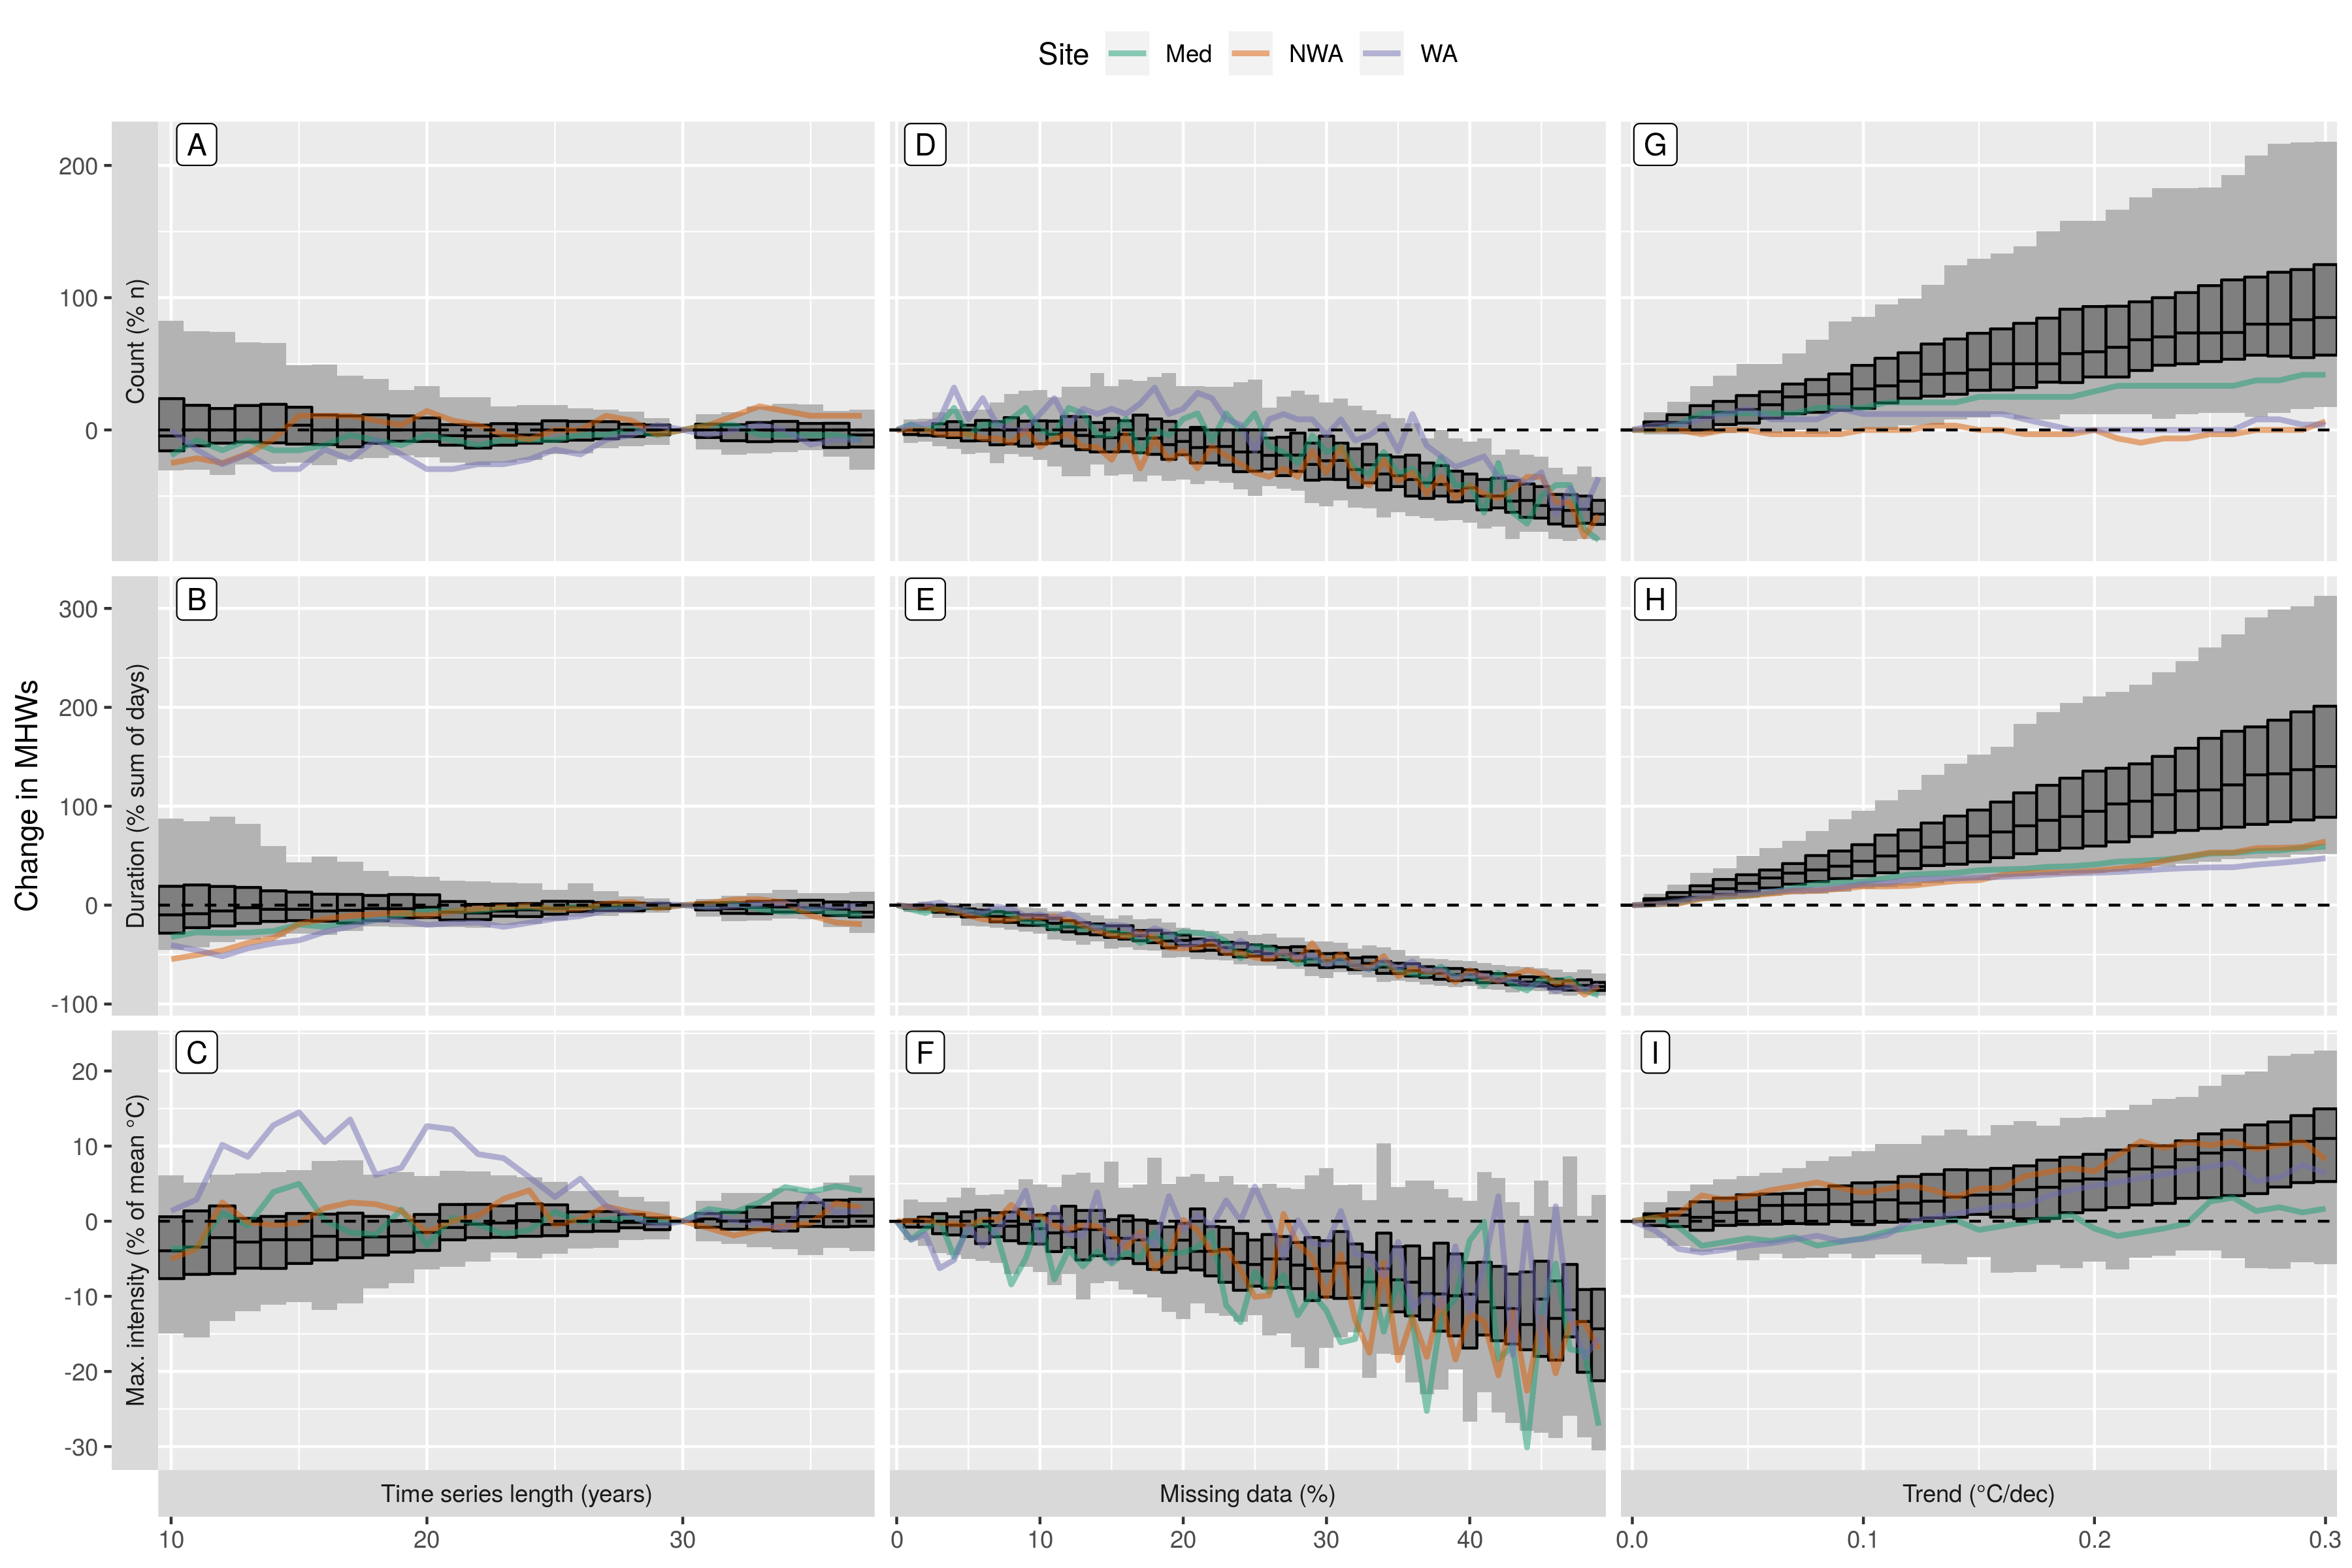
\includegraphics{../LaTeX/fig_2.png}
\caption{Figure 1: The results from Kolmogorov-Smirnov (KS) tests on the
similarity of distributions of MHW results given different sub-optimal
data conditions. The MHW properties are shown in different colours as
shown in the legend at the bottom of the figure. Each data point shows
the mean \emph{p}-value for each test at each step from the 100
re-sampled repetitions. The three columns show the different tests:
length (years), missing data (proportion), and added trend (°C/dec). The
three rows show the three reference time series: Med = Mediterranean,
NW\_Atl = North West Atlantic, WA = Western Australia. The x-axis shows
the value of the sub-optimal test and is different for each column. The
y-axis shows the range of mean \emph{p}-values from 1.0 (exact same) to
0.0 (completely different), with a horizontal dashed red line at 0.05
(statistically significantly different). Any points at or below the the
0.05 line are highlighted with red squares}
\end{figure}

The left hand column in Figure 2 shows the effect that shortening a time
series length has on the duration and max. intensity of the focus MHW
for the original data (not re-sampled) from each reference time series.
Because the shortening of a time series tends to increase the 90th
percentile threshold by making it more vulnerable to outliers, we see
that the shorter a time series becomes, the less the max. intensity and
duration of the MHWs become (Figure 2; bottom and middle panels). We
also see that the Western Australia (WA) and North West Atlantic
(NW\_Atl) MHWs are very quickly cut up into 2 or more MHWs due to the
rising 90th perc. threshold (Figure 2; top panel). The Mediterranean
(Med) MHW isn't affected much by time series length as it has little
fluctuation. Meaning it goes up and comes down, with no dips in the
middle like the other two reference MHWs.

\begin{figure}
\centering
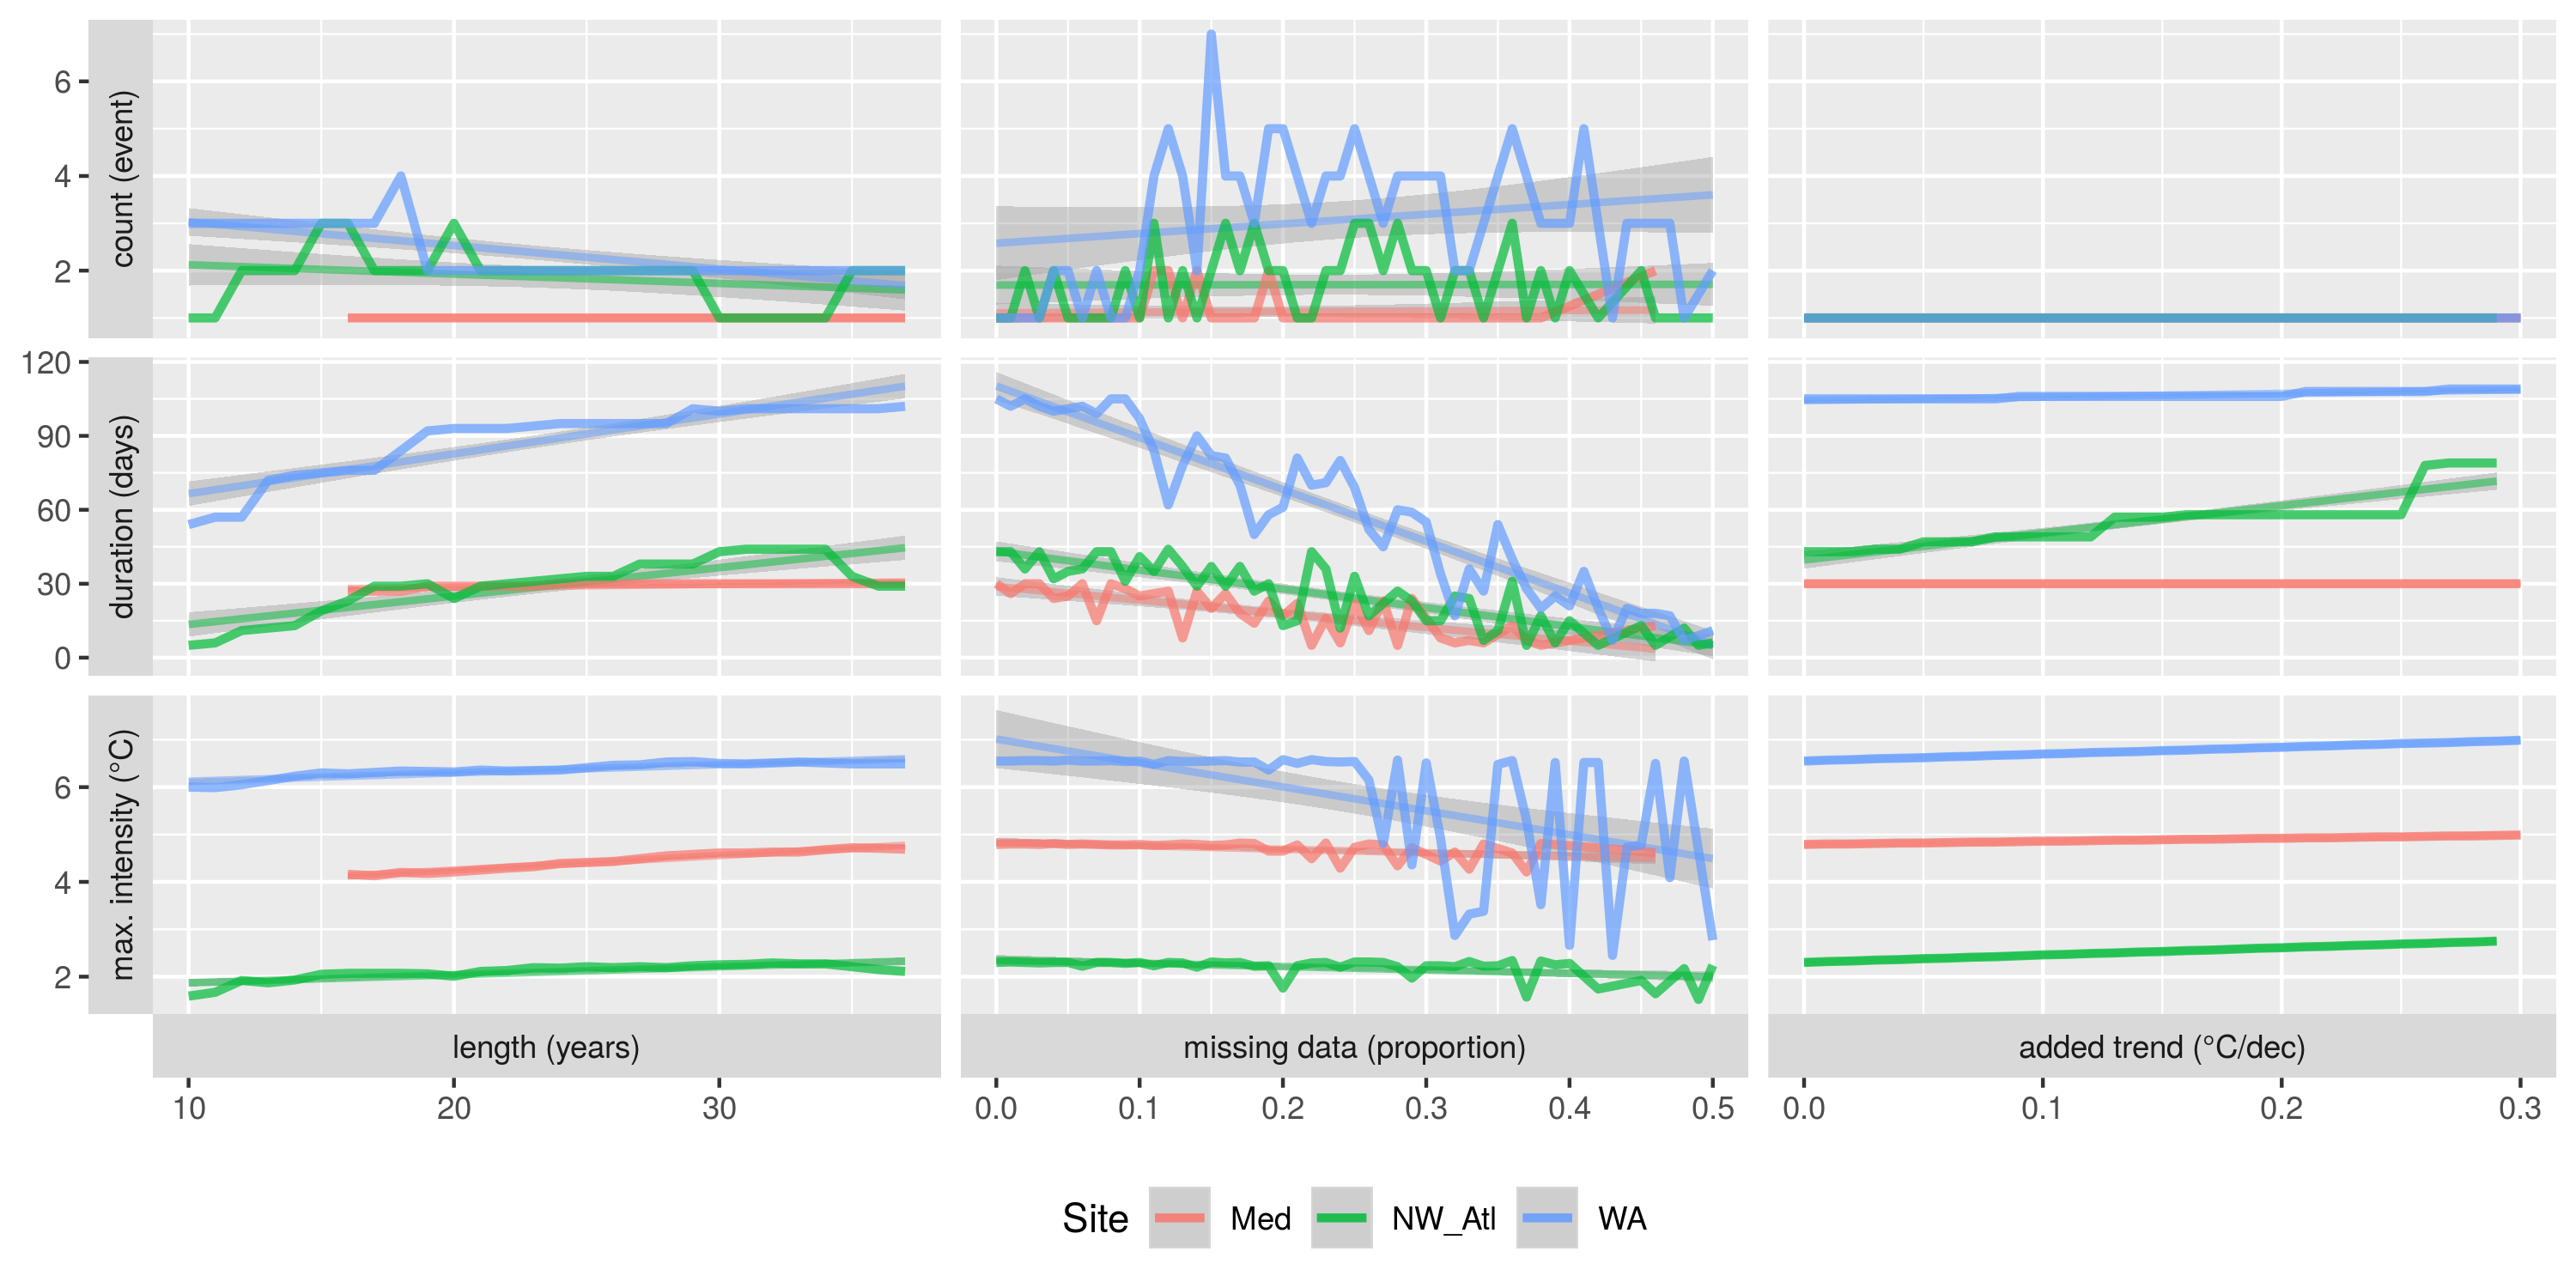
\includegraphics{../output/effect_event.png}
\caption{Figure 2: the effect of the three tests (columns) on the three
most relevant metrics (rows). Each panel has three lines, one for each
of the reference time series, shown in the legend at the bottom of the
figure. These are the original data, not the randomly re-samplef time
series from Question 1 . The lines track the change of just one metric
for just one MHW as the data are made increasingly sub-optimal, as shown
along the x-axes. The y-axes show the unit of measurement for each
metric. The top row, ``count (event)'' shows if the MHW is being chopped
up into multiple smaller MHWs due to changes in the values along the
x-axes.}
\end{figure}

When looking globally in Figure 3 we see that\ldots{}

\begin{figure}
\centering
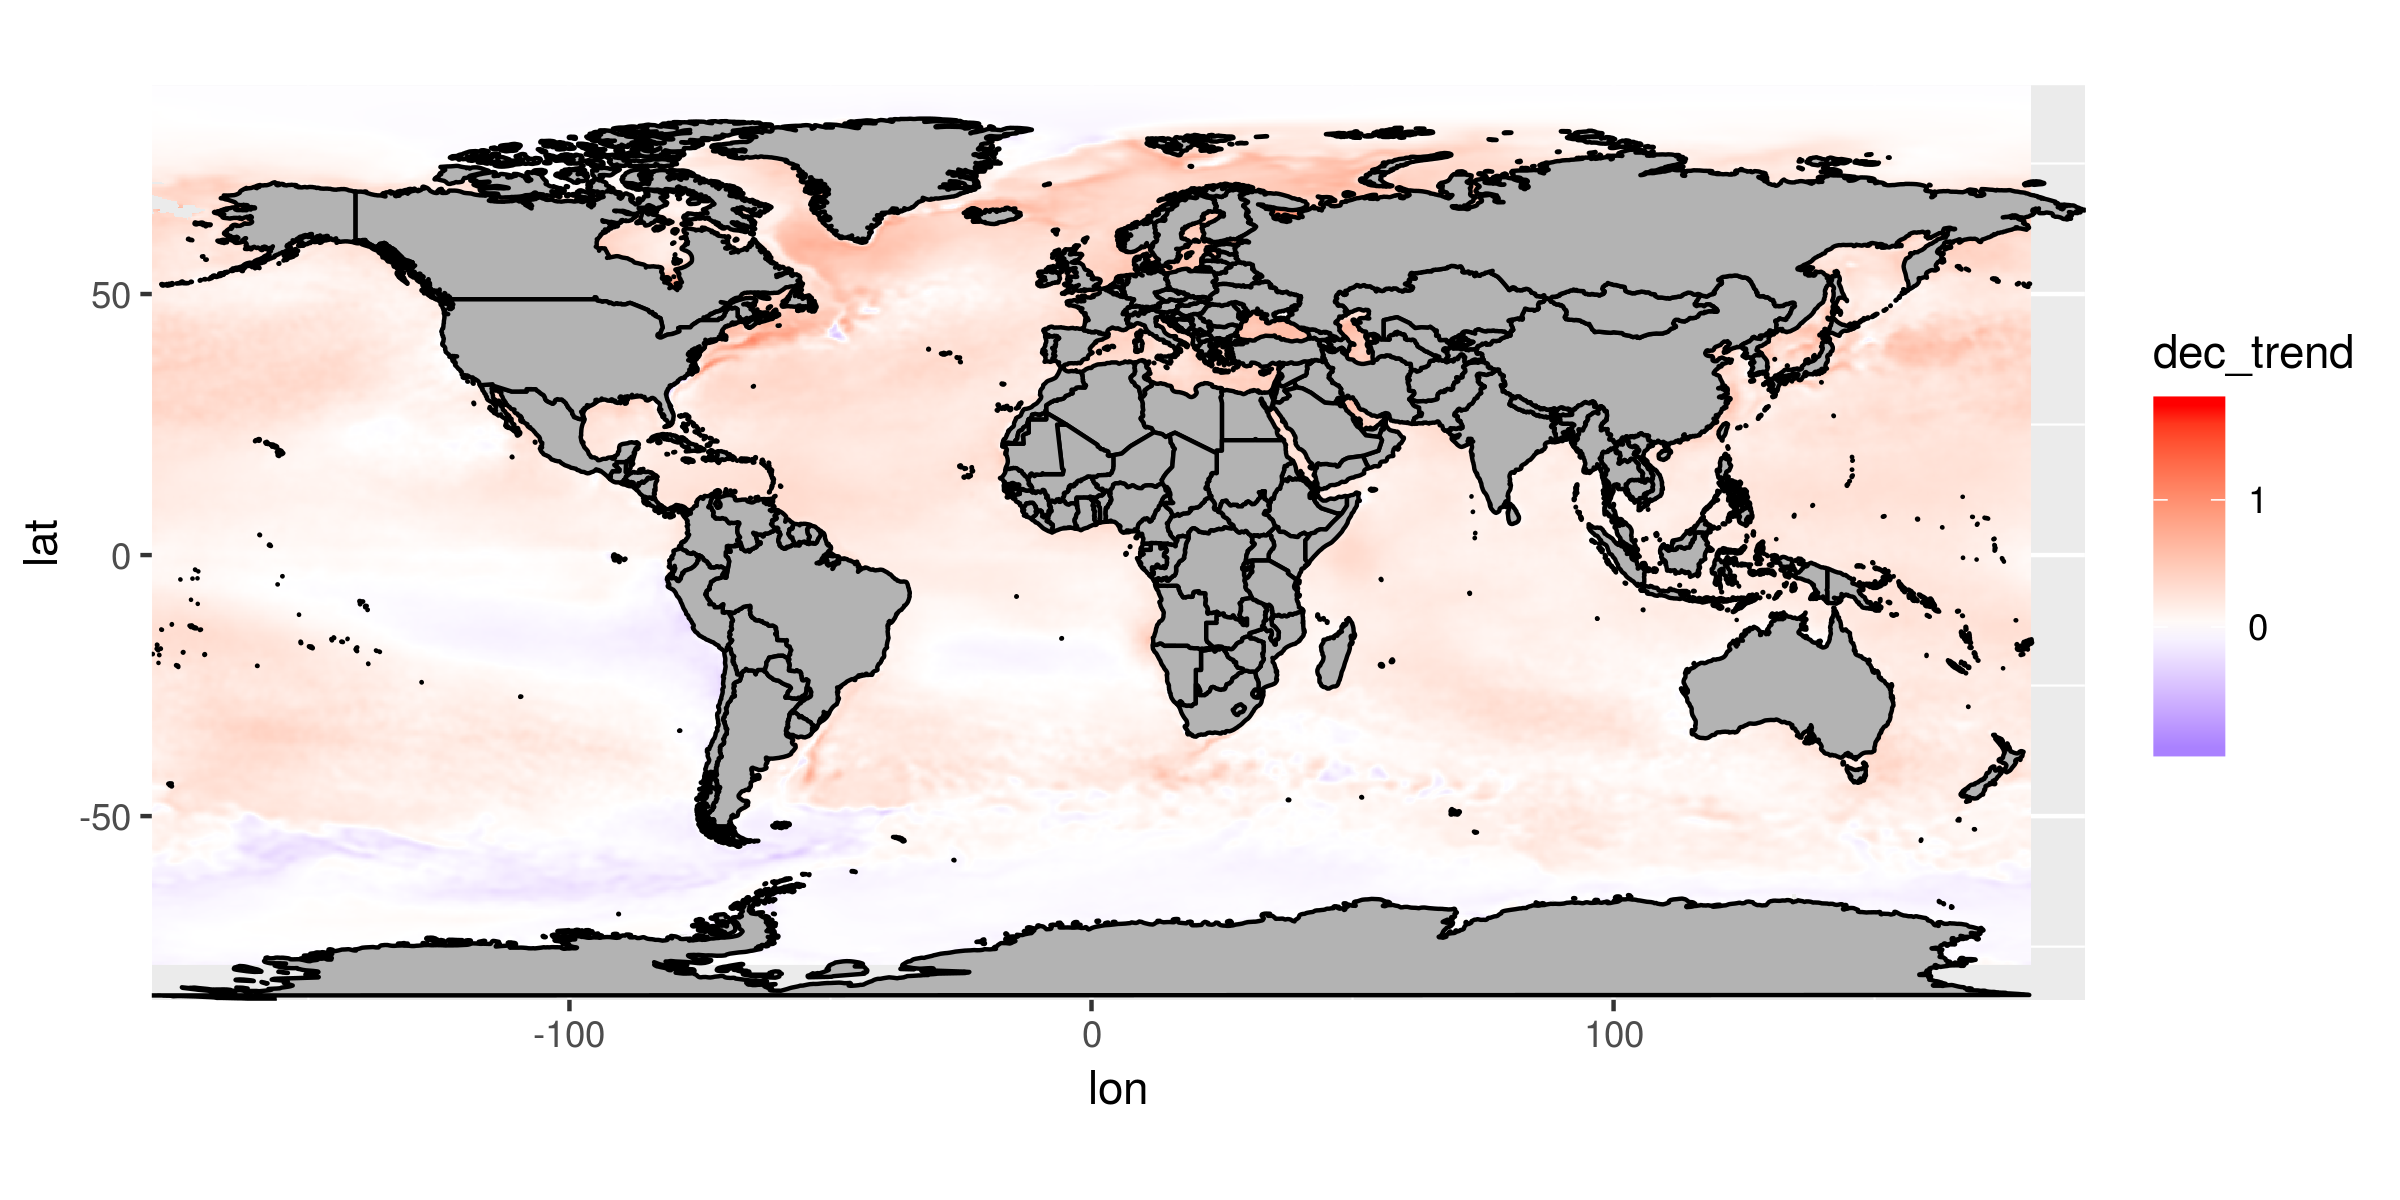
\includegraphics{../output/global_dec_trend_plot.png}
\caption{Figure 3: Global results placeholder}
\end{figure}

\hypertarget{missing-data}{%
\subsection{Missing data}\label{missing-data}}

(RWS: Please note that the write up in this section reflects the results
for missing data only from 0 -- 50\%. I've not had time since flying to
Texas to interpret the output of the effect of missing data up to 99\%)

The effects of missing data on MHW results is very pronounced. The
middle column of Figure 1 shows how quickly the results approach a level
of significant difference. The values most affected are the threshold
climatology, the duration of the MHWs, and the proportions of MHW days
in the moderate \& strong categories. The maximum intensities of the
MHWs are also affected, but at 50\% missing data these did not become
significantly different from the control time series. The proportion of
severe or extreme days were not affected by missing data as they were
already so rare or non-existent outside of the WA time series. The
seasonal signal was affected very little by large proportions of missing
data.

In the middle column of Figure 2 we see the effect that increasing
proportions of missing data have on the focus MHW. The lines seen in
these middle panels are very jagged because the missing data at each
step was only calculated once. This was done intentionally to highlight
the range that this randomness can have on the results. On the bottom
middle panel of Figure 2 we see that missing data can have very little
effect, or potentially an enormous effect, depending on the shape of the
MHW. The WA event has a very pronounced peak, so when larger proportions
of data are missing we see how massive the effect can be. The maximum
intensity measured in the control time series is 6.5°C, but we see that
because very few days of this MHW were so intense, increasing
proportions of missing data become more likely to delete the top of the
event. In the NW\_Atl event we see a gradual downward trend in the
maximum intensity because the event is more gradual in its ascent and
descent from the maximum. It is more plateau shaped. The effect on the
Med events appears to be the least pronounced, but upon closer
inspection we may see that the trend line ends at 41\% missing data
because enough of the event has been removed as to no longer exist.
Consider that this was one of the largest events recorded in the
Mediterranean at the time so it is no small comment that greater than
40\% missing data can completely remove the existence of an ecologically
damaging MHW.

In the middle panel of Figure 2 we see how the duration of the MHWs are
all negatively impacted by missing data, with the longer duration MHW
(WA) impacted much more than the shorter (NW\_Atl \& Med) MHWs. Even
though the decrease in duration due to missing data is very rough, we
see that it follows a linear trend and can therefore be predicted for
within a certain range of error.

The top middle panel of Figure 2 shows how many individual MHWs the
focus MHW is cut up into as missing data increase. At higher rates of
missing data the long NW\_Atl MHW is cut up into as many as six separate
MHWs.

\hypertarget{long-term-trends}{%
\subsection{Long-term trends}\label{long-term-trends}}

(RWS: Please note that the write up in this section reflects the results
for added decadal trends only from 0.00 -- 0.30C/dec. I've not had time
since flying to Texas to interpret the output of the effect of missing
data up to 0.50C/dec)

When adding a linear trend to the reference time series we see that it
created statistically significantly different climatologies at an
exponential rate (Figure 2; right column). The effect an added decadal
trend had on the other MHW results was roughly linear, and never
produced results significantly different from the control time series
(Figure 2). The maximum intensity and duration of events were affected
more than the proportions of days spent in the four categories.

The right hand column of Figure 2 shows how our focus MHWs were affected
by added decadal trends to the de-trended reference time series. We see
in the top panel that decadal trends never caused the focus MHW to be
dissected into multiple events. In the middle panel we see that the
duration of the events are affected differently by the added decadal
trend. The Med shows practically no effect, the NW\_Atl has a very
slight increase, whereas the WA event sees a massive increase with two
conspicuous jumps. The effect that the decadal trend has on the maximum
intensity of each event is a simple linear function of the decadal trend
and where in the time series the event occurs. The slope for the
increase in maximum intensity for the Med MHW is more shallow than the
other two because this MHW occurred in 2003, as opposed to 2010 (WA) and
2012 (NW\_Atl).

\hypertarget{fixes}{%
\subsection{Fixes}\label{fixes}}

(The interpretation of the fixes only goes through to 50\% at the
moment, because of Texas.)

The fixes proposed for shorter time series may have been beneficial for
time series under 15 years in length, but the correction they provided
was not consistent (Figure 4). The larger issue cause by a short time
series is the amount that the centre of the climatology increases or
decreases, more so than the increase in variability caused. This is not
something that can be controlled for \emph{a-priori} and is better
controlled for in a \emph{post-hoc} manner along the same lines as the
proposed fix for decadal trends (see below).

\begin{figure}
\centering
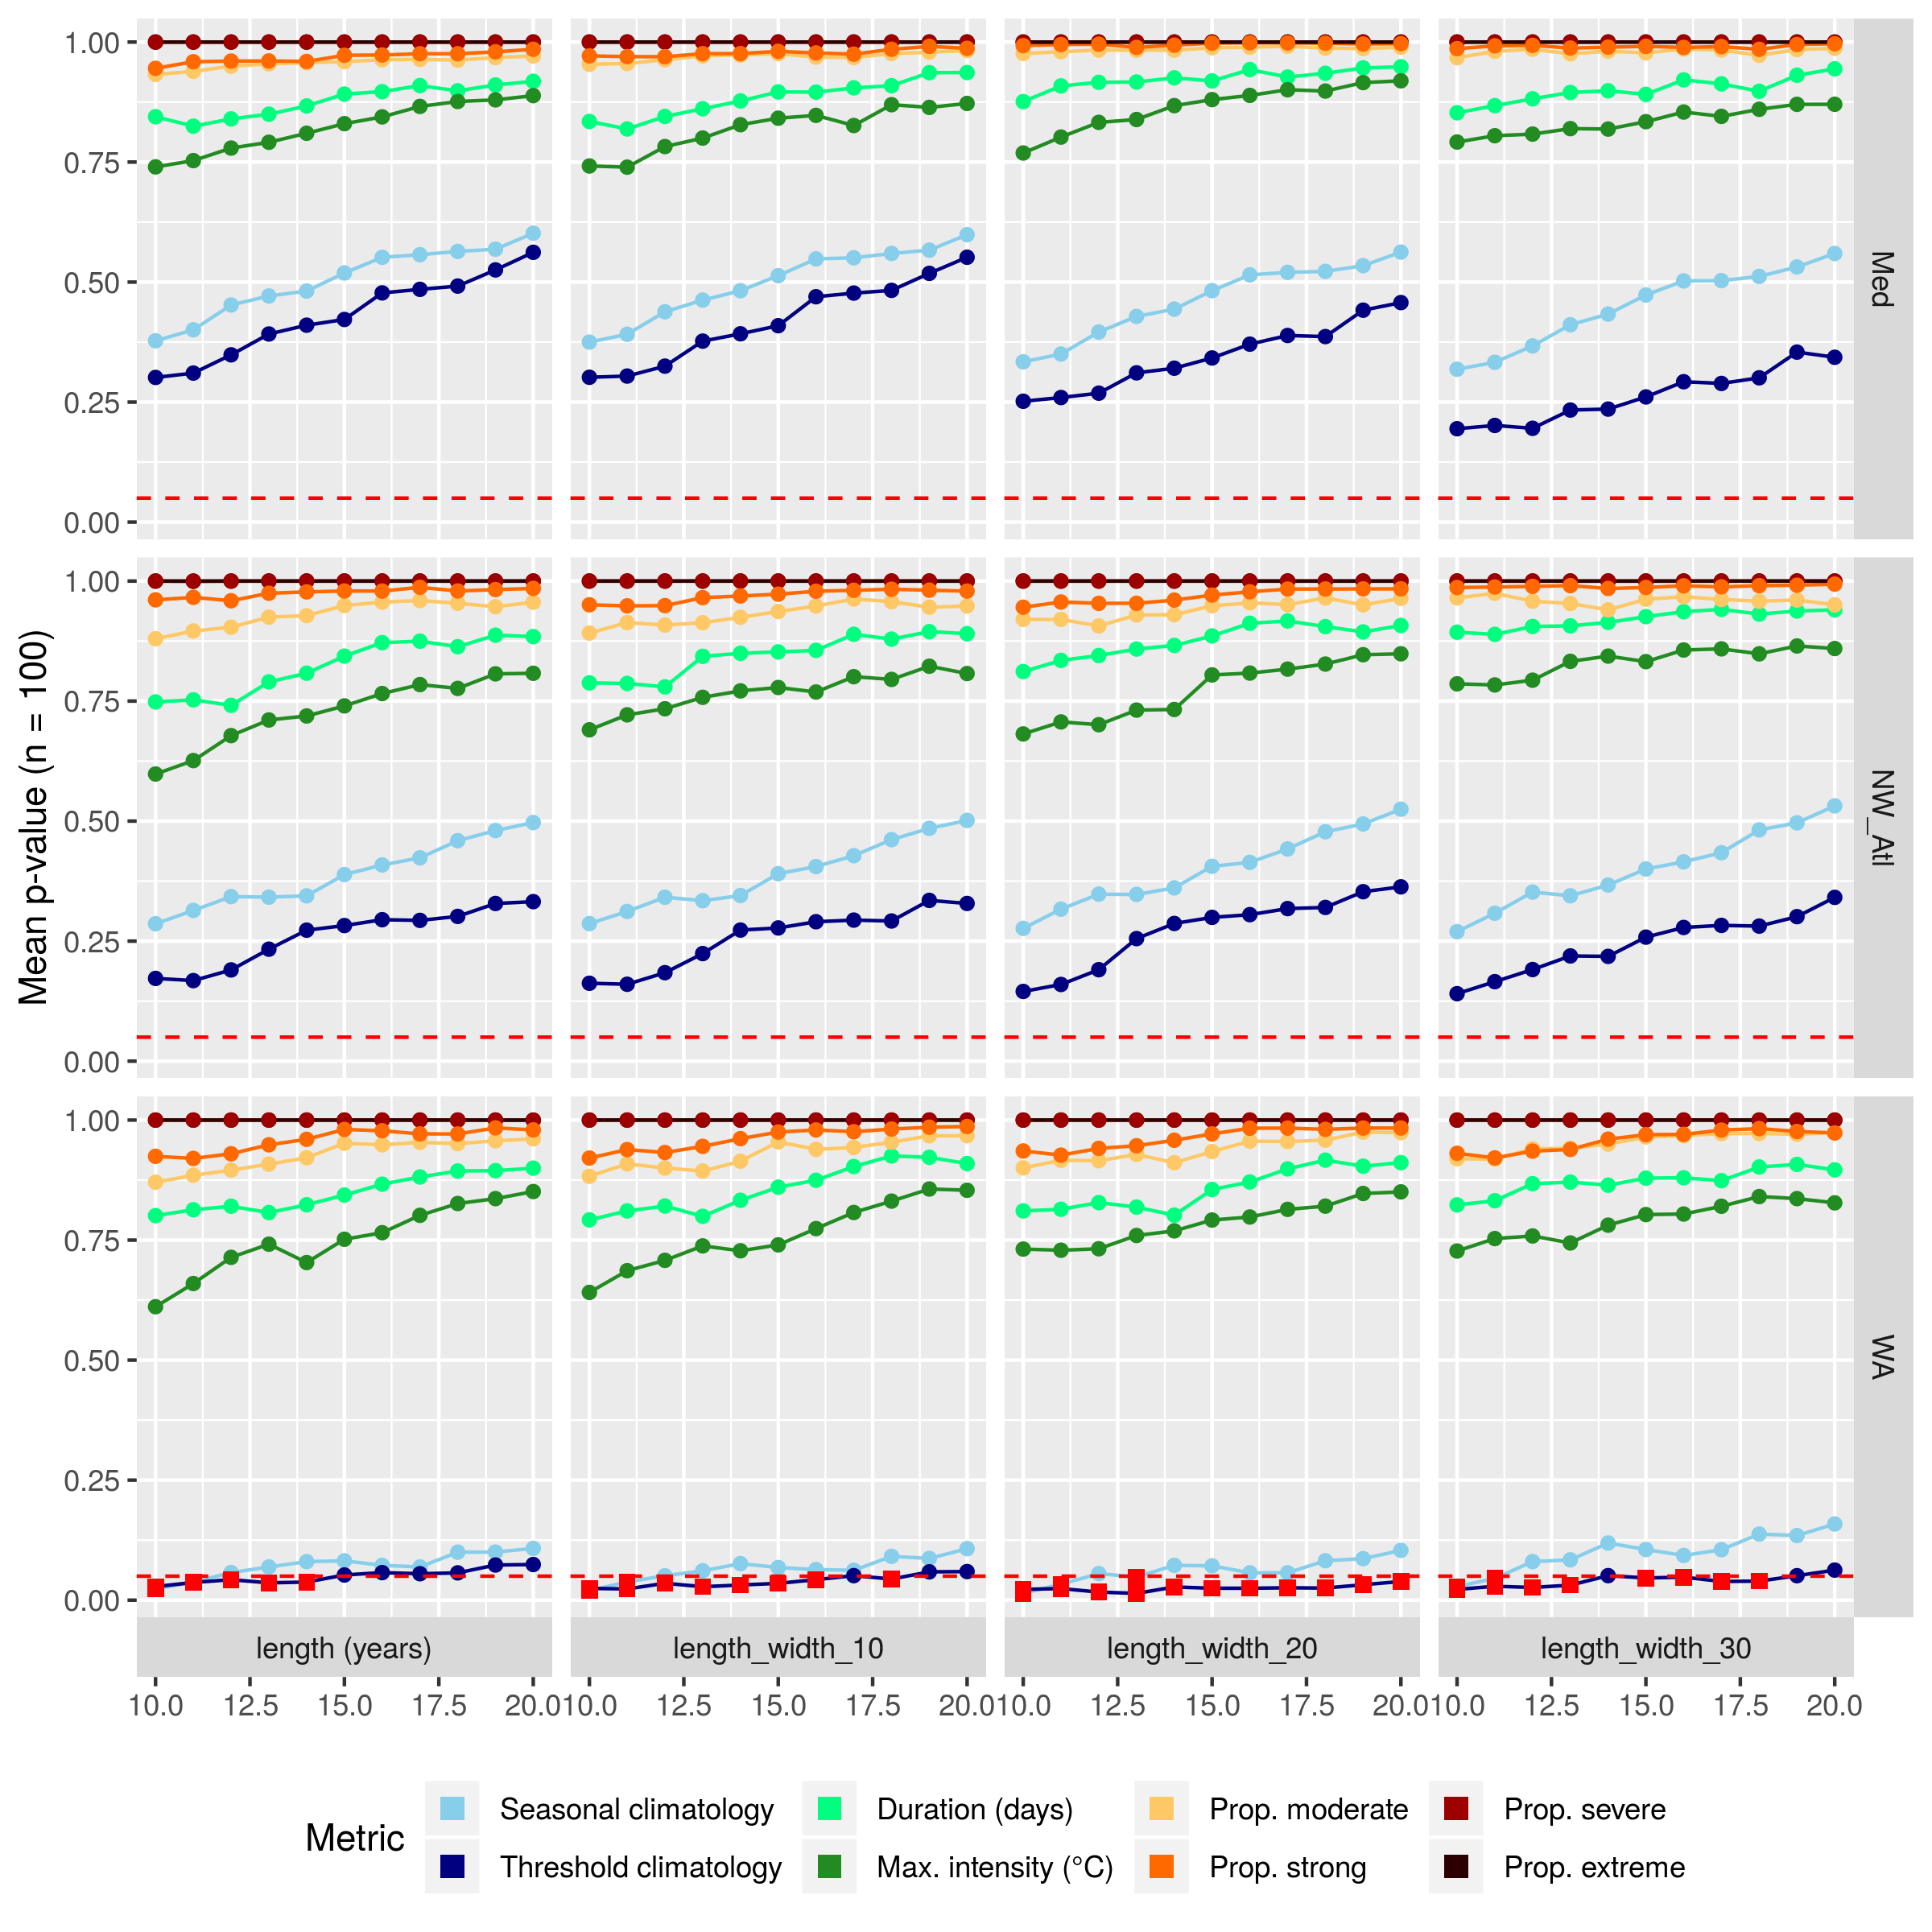
\includegraphics{../output/fig_2_length_only.png}
\caption{Figure 4: The short time series fixes. (RWS: I'm thinking that
this isn't useful to show and can rather just be mentioned.)}
\end{figure}

The linear interpolation of missing data was very effective and allows
for the use of time series missing much more than 50\% of their data, as
shown in Figure 5. Assuming of course that there is not so much missing
data that there are no representative days of the MHW that one may be
wanting to study/isolate.

\begin{figure}
\centering
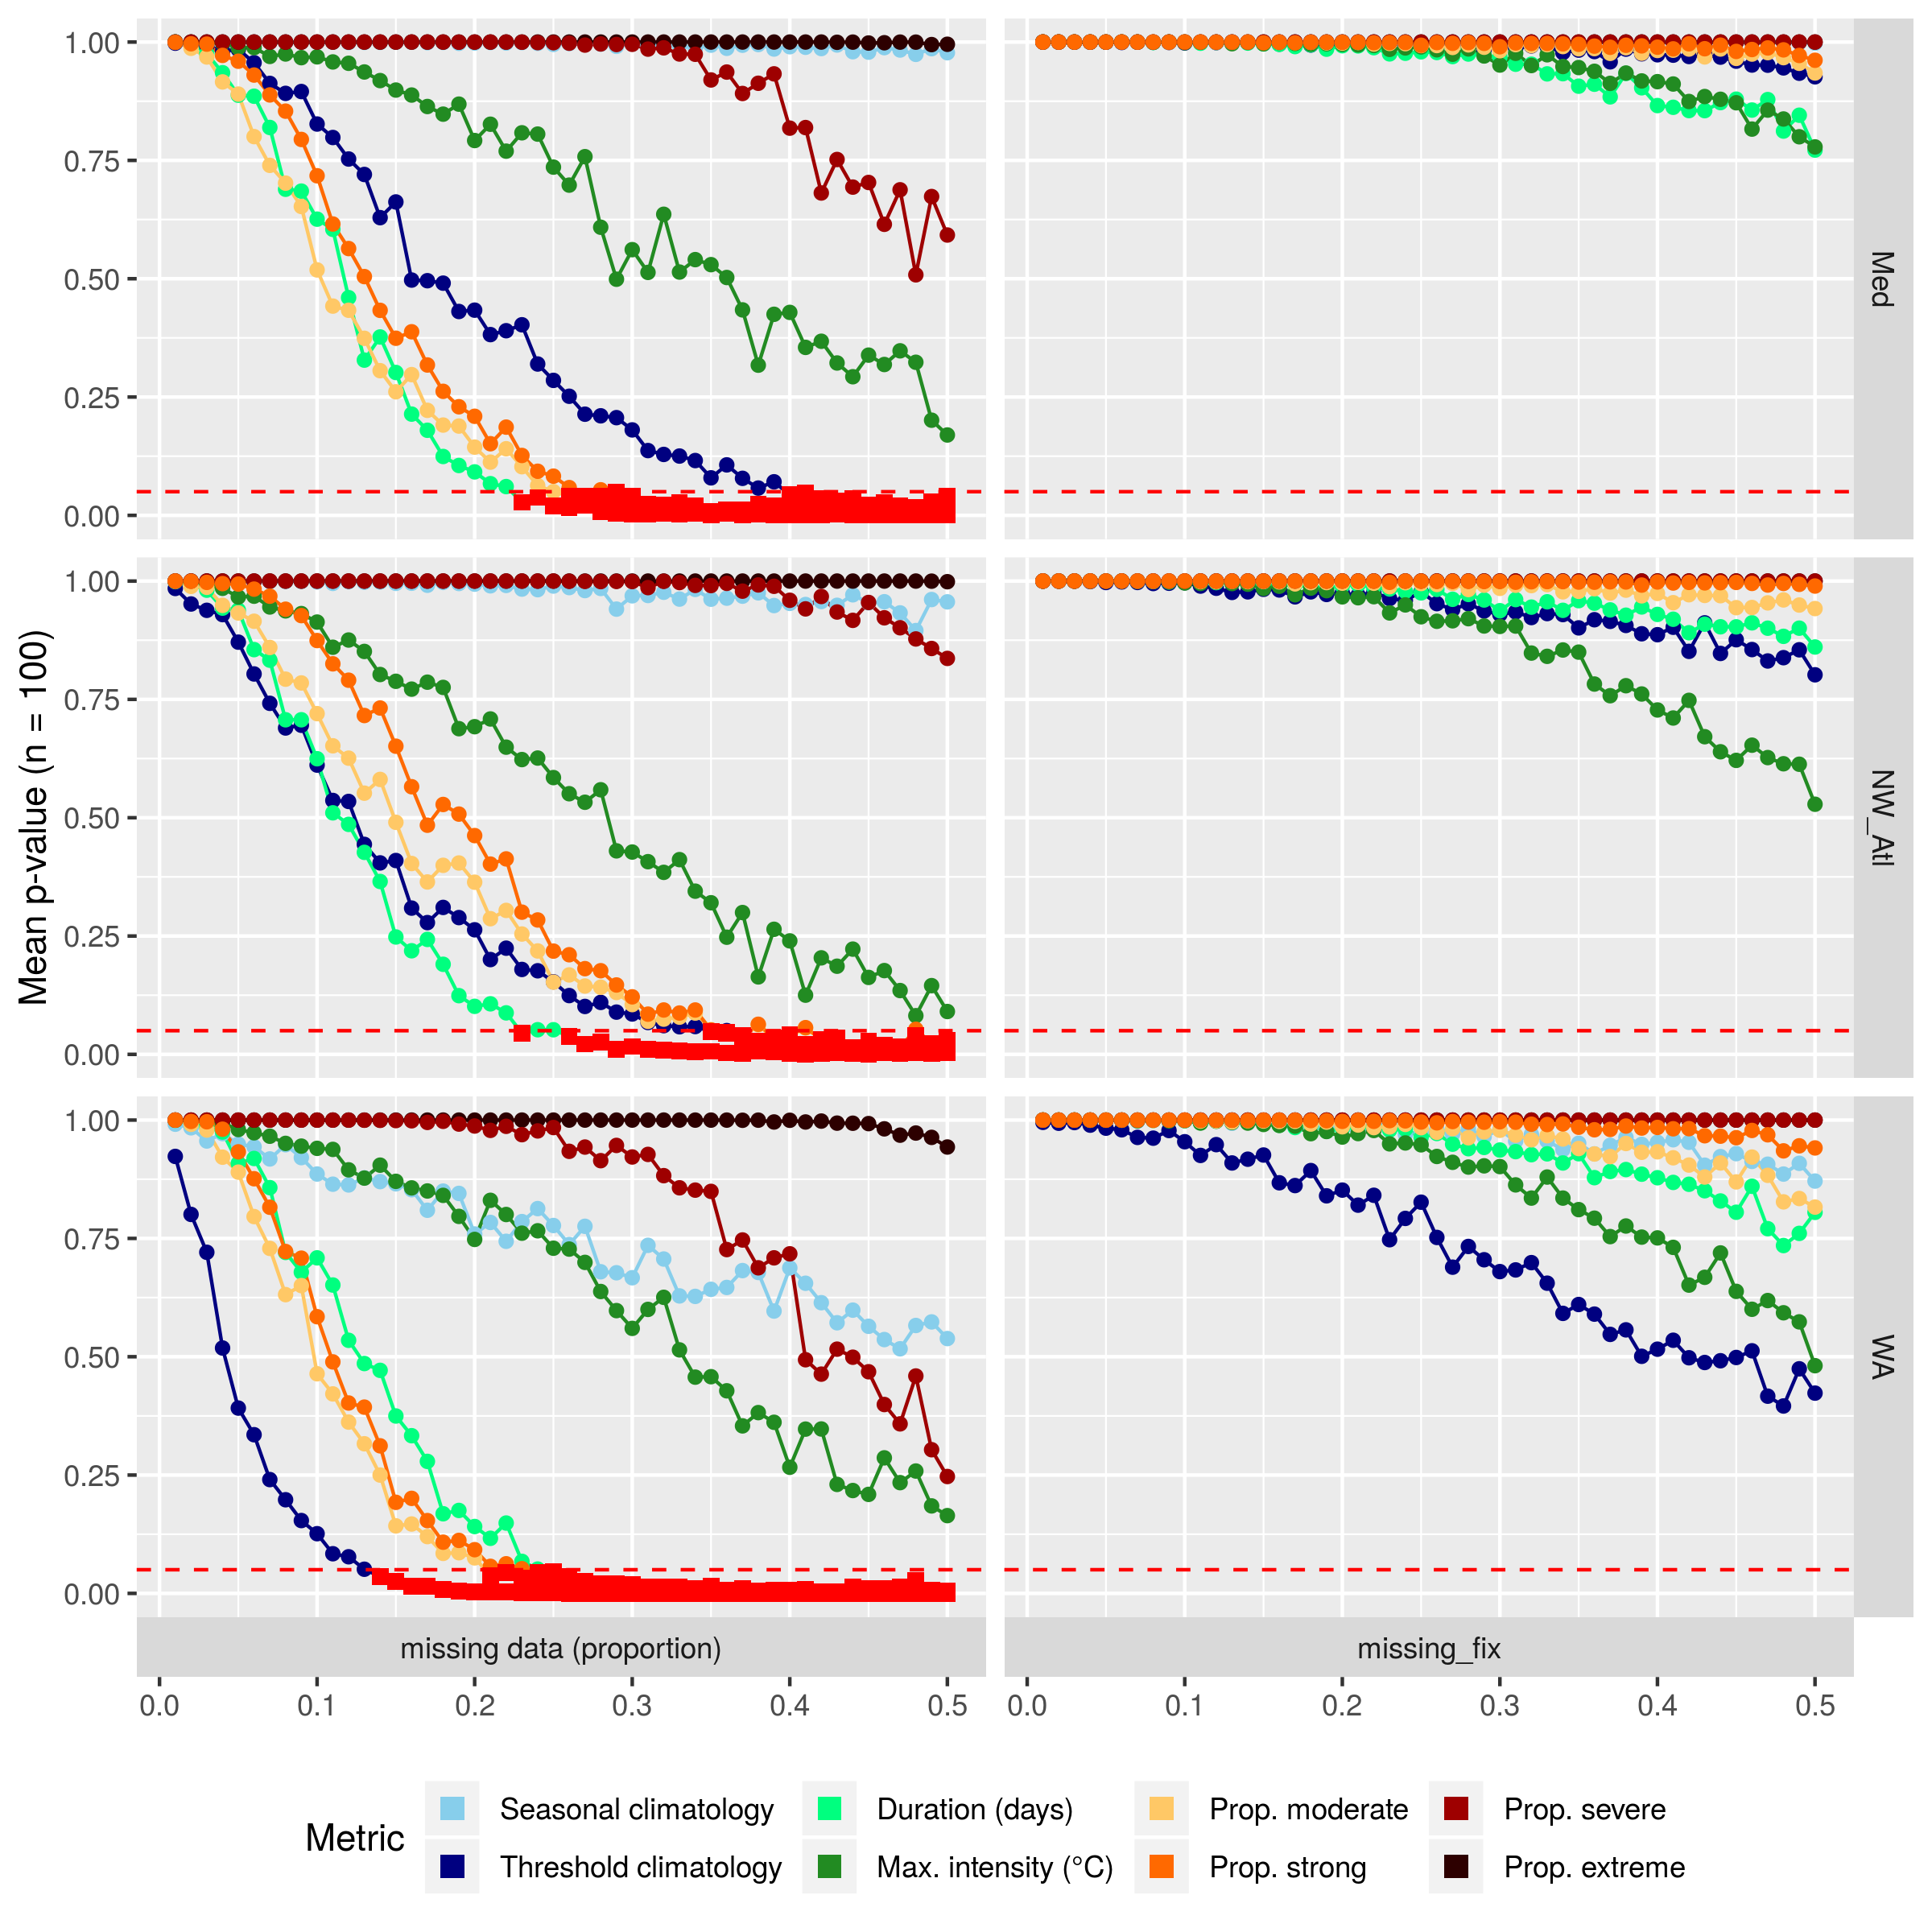
\includegraphics{../output/fig_2_missing_only.png}
\caption{Figure 5: The linear interpolation fixes.}
\end{figure}

We can see in Figure 3 that the effect that the decadal trend has on the
max. intensity of an event is a function of the slope of the trend and
the year during which the event took place. Knowing this we are able to
apply a \emph{post-hoc} correction to our results, as shown in Figure 6.

(RWS: This must still be done.)

\hypertarget{discussion}{%
\section{Discussion}\label{discussion}}

An investigation into the effects that sub-optimal data have on MHW
results revealed that the are certain thresholds that one may operate at
before having concern that ones results may not be usable. For time
series length one may use time series as short as 15 years before
needing to be concerned with the accuracy of the climatology results,
and 11 years for the accuracy of the MHW event metrics. The fix for the
effect of a short time series is complicated but if one is able to infer
the decadal trend in seawater temperature in the region of interest it
may be possible to improve the accuracy of the results. The MHW
algorithm proved to be resilient to missing data and so long as one does
not have particularly large gaps (e.g.~greater than a week at a time),
time series missing as much as 25\% of their data may be used without
concern. A simple correction for missing data is to linearly interpolate
over the gaps. It is not however recommended to do this as more than
40\% of missing data begins to dramatically distort the algorithms
ability to accurately create metrics for individual MHWs. The decadal
trends in times series very rapidly affect the creation of
climatologies, so whenever fewer than 30 years of data are used for the
climatology period one cannot say with any confidence that the results
are accurate. That being said, normal ranges of decadal trends (e.g.~0.1
-- 0.3C/dec) do not have a significant effect on the accurate detection
of MHWs. Furthermore, the effect of decadal trends is very predictable
and when taken with time series length and the year in which an event in
question has occurred it is possible to provide a confidence interval
around the metrics of the MHW.

From a high level view we can see that the panels in each column of
Figure 2 look similar, meaning that all three reference time series
responded similarly to the testing. The panels in each row appear to
differ much more, meaning that the different sub-optimal tests have more
of an effect on the results than the time series being measured. Missing
data have the largest effect on a time series, with length having the
smallest effect, but also the least predictable. We also see that the
seasonal and threshold climatologies tend to become significantly
different more quickly than the other metrics, with the exception that
the seasonal climatologies are affected very little by missing data.
Lastly we see that MHW duration and maximum intensity are affected more
quickly by time series length and added trend than the proportion of
days MHWs spend within a given category. The exception being that the
proportion of days of a MHW in moderate or strong categories is affected
more quickly by missing data. We also see in Figure 2 that none of the
trend lines have opposite slopes (i.e.~positive vs.~negative), but that
the degree of the angle of the slopes for a few of the panels are
clearly different.

The concept to consider with the increase in duration from added decadal
trends is that the decadal trend increases the temperatures in the time
series ``faster'' than the 90th perc. threshold. So as the decadal trend
increases, the MHW effectively spreads outwards. If the rate of
onset/decline for the MHW was gradual (e.g.~the NW\_Atl event) it will
increase in duration more rapidly. If the rate of onset/decline was more
rapid (e.g.~the Med event), then the duration of the MHW won't change
much with a larger decadal trend. The interesting line here is the WA
MHW. We can see that twice the duration of the event jumps rapidly. This
is because as the MHW spreads outward it encounters and engulfs two
other smaller MHWs and grows in duration.

The fact that, even the the results are similar, there is still a broad
range across them shows that one must always exercise caution when using
a sub-optimal time series. But that with a healthy dose of caution there
is still much that can be done to ameliorate the issues outlined in the
results. To this end we may look to the global results to see where the
patterns in the effects of sub-optimal data on MHW results hold up best,
and where they break down.

(RWS: A paragraph here about what the global results show us. And how we
can use that to advise on best practices when correcting for time series
length + decadal trend.)

\hypertarget{conclusions}{%
\section{Conclusions}\label{conclusions}}

(RWS: It would be good to show the bulleted advise on correction in the
conclusions.)

We have shown here that researchers must not shy away from the use of
sub-optimal time series when the situation calls for it, such as coastal
research or sub-surface analyses. Time series length may have an
unpredictable effect on MHW results, but this may be corrected for
within reason, and we have shown that time series lengths as short as 10
years are still useful for MHW research. Any shorter than this and the
realtionship between time series length and the effect on MHW metrics
becomes too unpredictable to provide any corrections with confidence. We
have however shown that MHW results from time series shorter than 10
years will likely not be significantly different from 30 year time
series. Missing data has a larger effect, but is less of a concern as
linear interpolation can largely fix the challenges this creates, up to
a threshold of 40\% missing data. Lastly, the errors introduced by
long-term trends in the data are the most predictable and when taken
with time series length may be corrected for as well. The MHW detection
algorithm is very robust and we have shown here that one may be
confident in the inter-comparability of ones results when using time
series within a generous range.

\hypertarget{references}{%
\section*{References}\label{references}}
\addcontentsline{toc}{section}{References}

\hypertarget{refs}{}
\leavevmode\hypertarget{ref-Baumgartner1992}{}%
Baumgartner, TR. 1992. ``Reconstruction of the History of the Pacific
Sardine and Northern Anchovy Populations over the Past Two Millenia from
Sediments of the Santa Barbara Basin, California.'' \emph{CalCOFI Rep}
33: 24--40.

\leavevmode\hypertarget{ref-Hobday2016}{}%
Hobday, Alistair J, Lisa V Alexander, Sarah E Perkins, Dan A Smale,
Sandra C Straub, Eric CJ Oliver, Jessica A Benthuysen, et al. 2016. ``A
Hierarchical Approach to Defining Marine Heatwaves.'' \emph{Progress in
Oceanography} 141. Elsevier: 227--38.

\leavevmode\hypertarget{ref-Hobday2018}{}%
Hobday, Alistair J, Eric CJ Oliver, Alex Sen Gupta, Jessica A
Benthuysen, Michael T Burrows, Markus G Donat, Neil J Holbrook, et al.
2018. ``Categorizing and Naming Marine Heatwaves.'' \emph{Oceanography}
31 (2). JSTOR: 162--73.

\leavevmode\hypertarget{ref-Oliver2018}{}%
Oliver, Eric CJ, Markus G Donat, Michael T Burrows, Pippa J Moore, Dan A
Smale, Lisa V Alexander, Jessica A Benthuysen, et al. 2018. ``Longer and
More Frequent Marine Heatwaves over the Past Century.'' \emph{Nature
Communications} 9 (1). Nature Publishing Group: 1324.

\leavevmode\hypertarget{ref-WMO2011}{}%
Organization, World Meteorological. 2011. \emph{Guide to Climatological
Practices}. World Meteorological Organization (WMO).

\leavevmode\hypertarget{ref-WMO2017}{}%
---------. 2017. \emph{WMO Guidelines on the Calculation of Climate
Normals}. World Meteorological Organization (WMO).

\leavevmode\hypertarget{ref-IPCC2014}{}%
Pachauri, Rajendra K, Leo Meyer, J van Ypersele, Sander Brinkman, Line
van Kesteren, Noëmie Leprince-Ringuet, and Fijke Van Boxmeer. 2014.
``Climate Change 2014 Synthesis Report.''

\leavevmode\hypertarget{ref-Philander1983}{}%
Philander, S George H. 1983. ``El Nino Southern Oscillation Phenomena.''
\emph{Nature} 302 (5906). Nature Publishing Group: 295.

\leavevmode\hypertarget{ref-Reynolds2007}{}%
Reynolds, Richard W, Thomas M Smith, Chunying Liu, Dudley B Chelton,
Kenneth S Casey, and Michael G Schlax. 2007. ``Daily
high-resolution-blended analyses for sea surface temperature.''
\emph{Journal of Climate} 20 (22). NOAA, Natl Climatic Data Ctr,
Asheville, NC 28801 USA: 5473--96.

\leavevmode\hypertarget{ref-Salinger2016}{}%
Salinger, J., A.J. Hobday, R.J. Matear, T.J. O'Kane, J.S. Risbey, P.
Dunstan, J.P. Eveson, et al. 2016. ``Chapter One - Decadal-Scale
Forecasting of Climate Drivers for Marine Applications.'' In, edited by
Barbara E. Curry, 74:1--68. Advances in Marine Biology. Academic Press.
\url{https://doi.org/https://doi.org/10.1016/bs.amb.2016.04.002}.

\leavevmode\hypertarget{ref-Schlegel2018}{}%
Schlegel, Robert W, and Albertus J Smit. 2018. ``HeatwaveR: A Central
Algorithm for the Detection of Heatwaves and Cold-Spells.'' \emph{The
Journal of Open Source Software} 3: 821.

\leavevmode\hypertarget{ref-Smale2019}{}%
Smale, Dan A, Thomas Wernberg, Eric CJ Oliver, Mads Thomsen, Ben P
Harvey, Sandra C Straub, Michael T Burrows, et al. 2019. ``Marine
Heatwaves Threaten Global Biodiversity and the Provision of Ecosystem
Services.'' \emph{Nature Climate Change}. Nature Publishing Group, 1.

\leavevmode\hypertarget{ref-Zhao2019}{}%
Zhao, Zijie, and Maxime Marin. 2019. ``A Matlab Toolbox to Detect and
Analyze Marine Heatwaves.'' \emph{The Journal of Open Source Software}
4: 1124.


\end{document}
